\chapter{Programmation de l'OpenCR}

\section{Initialisation de l'IDE}
\label{init_ide}

\noindent Pour programmer la carte OpenCR, l'IDE Arduino sera utilisé. Il faut donc le télécharger ici : 
\url{https://www.arduino.cc/en/software/}

\noindent Une fois l'IDE installé et ouvert, aller dans \textbf{File} > \textbf{Preferences}, et ajouter le lien suivant : 

\url{https://raw.githubusercontent.com/ROBOTIS-GIT/OpenCR/master/arduino/opencr_release/package_opencr_index.json}

\noindent Dans la case \textit{URL de gestionnaire de cartes supplémentaires} :

\begin{figure}[H]
    \centering
    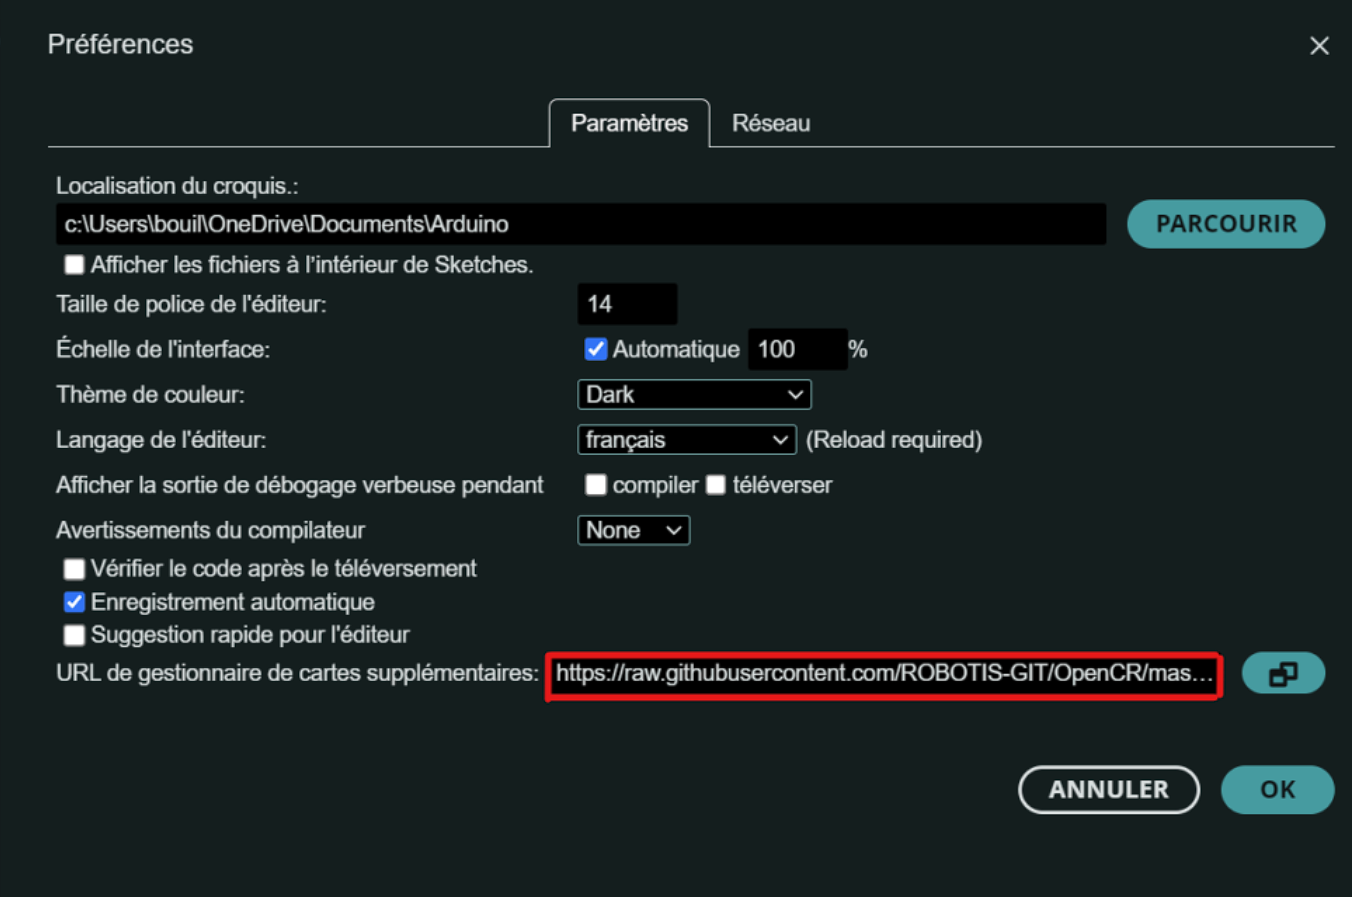
\includegraphics[width=1\textwidth]{Annexes/Mecanum_ROS2/OpenCR/pictures/addOpenCR.png}
    \caption{URL de gestionnaire de cartes supplémentaires}
\end{figure}

\noindent Plus de détails sont donnés ici : \url{https://emanual.robotis.com/docs/en/parts/controller/opencr10/}

\section{Programmation de la carte}

La bibliothèque \textit{Micro-ROS-Arduino} (\url{https://github.com/micro-ROS/micro_ros_arduino}) est utilisée pour programmer l'OpenCR. Elle permet notamment de communiquer avec la Raspberry PI et le Micro-Ros Agent si cette dernière est branché en USB avec l'OpenCR. Des exemples de code sont disponibles dans \textbf{File > Examples > micro\_ros\_arduino}. 

Ci-dessous est donné une explication de leur fonctionnement.

\subsection{Inclusion des bibliothèques}

\begin{lstlisting}[style=commandstyle]
#include <micro_ros_arduino.h>
#include <rcl/rcl.h>
#include <rcl/error_handling.h>
#include <rclc/rclc.h>
#include <rclc/executor.h>
\end{lstlisting}

\subsection{Création d'un nœud ROS}
\noindent La fonction \textit{rclc\_node\_init\_default} initialise un nœud ROS2, elle est à mettre dans le \textit{setup} :

\begin{lstlisting}[style=commandstyle]
rcl_node_t node;
rclc_support_t support;
RCCHECK(rclc_node_init_default(&node, "micro_ros_arduino_node", "", &support));
\end{lstlisting}

\subsection{Création d'un publisher et d'un subscriber}

\noindent Il faut mettre ces programmes dans le setup.
\begin{lstlisting}[style=commandstyle , caption={Création d'un Publisher}]
RCCHECK(rclc_publisher_init_default(
  &publisher,
  &node,
  ROSIDL_GET_MSG_TYPE_SUPPORT(std_msgs, msg, Int32),
  "micro_ros_arduino_node_publisher"));
\end{lstlisting}

\begin{lstlisting}[style=commandstyle ,caption={Création d'un Subscriber}]
RCCHECK(rclc_subscription_init_default(
  &subscriber,
  &node,
  ROSIDL_GET_MSG_TYPE_SUPPORT(std_msgs, msg, Int32),
  "micro_ros_arduino_subscriber"));
\end{lstlisting}
\vspace{-0.3cm}
\subsection{Callback}

\noindent Un \textit{callback} est attribué à un \textit{subscriber}, ce qui lui permet de récupérer les données sur un topic.

\begin{lstlisting}[style=commandstyle]
void subscription_callback(const void * msgin) {
  const std_msgs__msg__Int32 * msg = (const std_msgs__msg__Int32 *)msgin;
  digitalWrite(LED_PIN, (msg->data == 0) ? LOW : HIGH);
}
\end{lstlisting}

\subsection{Configuration d'un timer}
\noindent Permet de programmer un \textit{timer}, qui va organiser l’exécution des tâches à des intervalles réguliers.
\begin{lstlisting}[style=commandstyle]
const unsigned int timer_timeout = 1000; // Intervalle en ms
RCCHECK(rclc_timer_init_default(
  &timer,
  &support,
  RCL_MS_TO_NS(timer_timeout),
  timer_callback));
\end{lstlisting}

\subsection{Callback du timer}

\begin{lstlisting}[style=commandstyle]
void timer_callback(rcl_timer_t * timer, int64_t last_call_time) {
  if (timer != NULL) {
    RCSOFTCHECK(rcl_publish(&publisher, &msg, NULL)); // Publier le message
    msg.data++;
  }
}
\end{lstlisting}

\subsection{Configuration de l'exécuteur}

\noindent L'éxécuteur va, comme son nom l'indique, éxecuter les différents \textit{callback}
\begin{lstlisting}[style=commandstyle]
RCCHECK(rclc_executor_init(&executor, &support.context, 1, &allocator));
RCCHECK(rclc_executor_add_timer(&executor, &timer));
\end{lstlisting}

\noindent Par exemple, pour ajouter un \textit{subscriber} à l'éxecuteurs :

\begin{lstlisting}[style=commandstyle]
RCCHECK(rclc_executor_add_subscription(
  &executor,
  &subscriber,
  &msg,
  &subscription_callback,
  ON_NEW_DATA));
\end{lstlisting}

\subsection{Boucle principale}

\begin{lstlisting}[style=commandstyle]
RCSOFTCHECK(rclc_executor_spin_some(&executor, RCL_MS_TO_NS(100)));
\end{lstlisting}

\subsection{Programme pour robot Mecanum}

\noindent Les programmes Arduino pour les robots Mecanum sont disponibles ici : \url{https://github.com/watson67/mecanum/tree/main/holonome_mecanum_ros2}. Il faut mettre les 4 fichiers dans un même dossier, ouvrir \textit{holonome\_mecanum\_ros2.ino} dans l'IDE Arduino puis téléverser.


